\section{Introduction}
I have spent the majority of my time this week learning new things to support my knowledge about Deep Learning. I also tried to grasp the idea of Places365 framework and deploy it on my own computer as well as on the Google Colab.

\section{EPFL Deep Learning Course}
To gain more experience on Deep Learning area, I started learning EPFL Deep Learning course\cite{epfl} but unfortunately, I made it through without any taken notes. So lately I decided to start learning from the beginning and taking note with Jupyter at the same time. Until now, I finished 5 main lectures.
	
\textbf{\emph{Introduction and Tensor}}. The first lecture was about answering these questions what is deep learning, some history, what are the current applications. The lecturer also briefly introduced the most basic unit in PyTorch which was torch.Tensor; then using PyTorch to demonstrate linear regression problems.

\textbf{\emph{Machine learning fundamentals}}. The lecturer taught me about the theories of Empirical risk minimization, capacity, bias-variance dilemma, polynomial regression, k-means and PCA.

\textbf{\emph{Multi-layer perceptrons}}. The lecturer firstly taught about Linear classifiers, the perceptron concept, linear separability and feature extraction. Then we moved to Multi-Layer Perceptron, gradient descent and back-propagation techniques.

\textbf{\emph{Convolutional Networks and Autograds}}. This lecture was about the Generalized acyclic graph networks; the torch.autograd technique to simplify our works; batch processing technique in training state. The lecturer also introduced the idea of convolutional layers and pooling layers as well as knowledge about kernel. After all, I was taught how to use \emph{torch.nn.Module} from PyTorch to implement all of the cool things above practically.

	
\textbf{\emph{Optimization}}. In this lecture, the lecturer taught me about the Cross-entropy, L1 and L2 penalty to train a neural network. Then I was taught several techniques to optimize our works during designing and training our neural network such as vanishing gradient, weight initialization, Xavier's rule and loss monitoring. Finally I was taght to implement everything I had learnt so far by using \emph{torch.autograd.Function}.

During the learning process I had taken some notes and they could be found \href{https://gitlab.com/tlvu2697/epfl--ee559--deep-learning}{here on my GitLab}.

\section{CSAIL Places}
\subsection{Introduction}
The \href{http://places2.csail.mit.edu/}{Places} dataset was designed following principles of human visual cognition could be used to train artificial systems for high-level visual understanding tasks, such as scene context, object recognition, action and event prediction, and theory-of-mind inference. Thing that made this dataset more special than others was that the semantic categories of Places are defined by their function: the labels represented the entry-level of an environment. For example the dataset had different categories of bedrooms, or streets.

\subsection{Places Challenge}
The goal of this challenge was to identify the scene category depicted in a photograph. The data for this task came from the Places dataset.

For each image, algorithms would produce a list of at most 5 scene categories in descending order of confidence. The quality of a labeling would be evaluated based on the label that best matches the ground truth label for the image.

\subsection{Places365 Convolutional Neural Networks}
\subsubsection{Introduction}
Places365\cite{places365} provided several pre-trained CNN models in 2 different frameworks which were Caffe\cite{caffe} and PyTorch\cite{pytorch}. These models was train on the Places365-Standard dataset which had 1.8 million train images from 365 scene categories. With PyTorch framework, Places365 delivered 4 pre-trained model networks AlexNet\cite{alexnet}, ResNet18\cite{resnet}, ResNet50 and DenseNet161\cite{densenet} to work with.

\subsubsection{Demo}
Beside released CNN models, Places365 also provided Python code to run which could be found \href{https://github.com/CSAILVision/places365}{here on their GitHub}. After deploying the demo, I got these results by running on different Convolutional Neural Networks models.

We could clearly see how differently each model actually looks at the input image. The ResNet18 model only focused on one small spot on top of the waterfall to make decision. The ResNet50 instead mainly focused on 3 different spots to make decision, so maybe that was the reason why the certainty of conclusions are significantly low. The DenseNet161 model focused exactly where the waterfall was and also provided good conclusions. So I thought we should only use 2 models, ResNet18 for simplification or DenseNet161 for better conclusions (and Class Activation Map).


\begin{figure}[!ht]
\centering
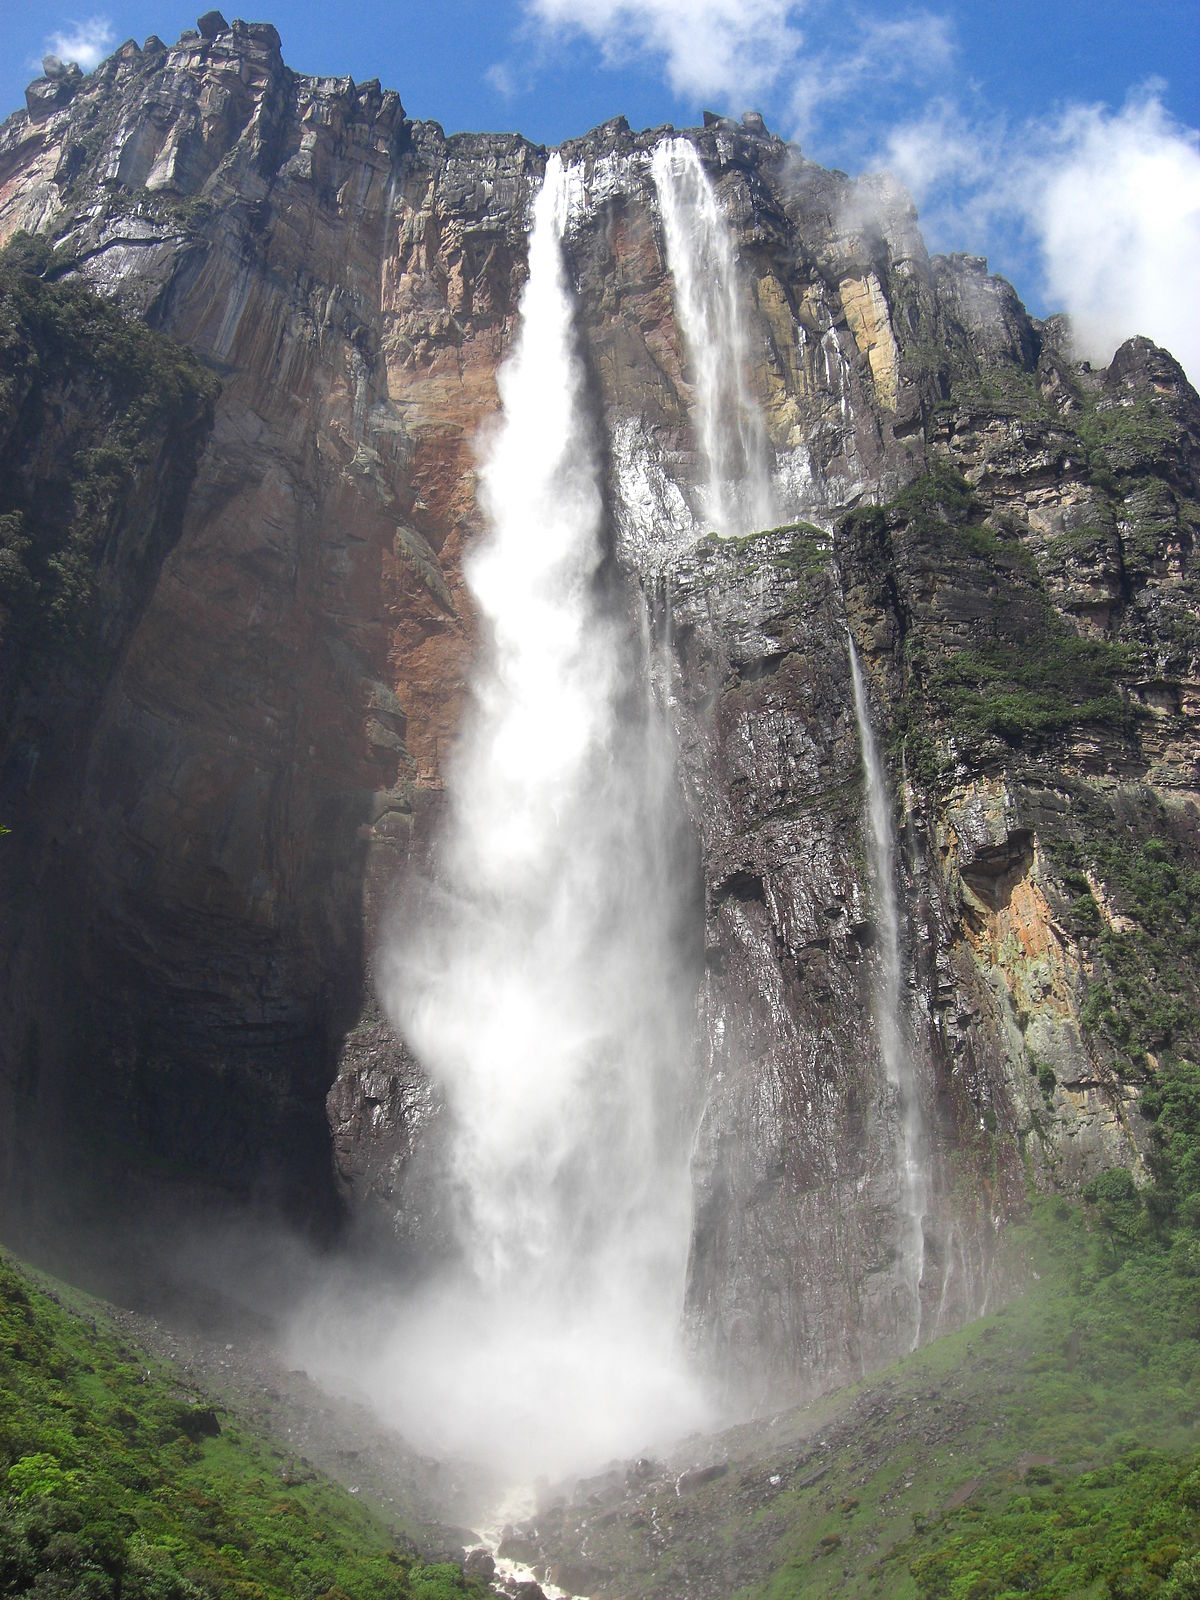
\includegraphics[width=0.4\textwidth,keepaspectratio]{week1-input.jpg}
\caption{Input image}
\end{figure}

\newpage
\begin{figure}[!ht]
\centering
\begin{subfigure}{0.7\textwidth}
  \centering
  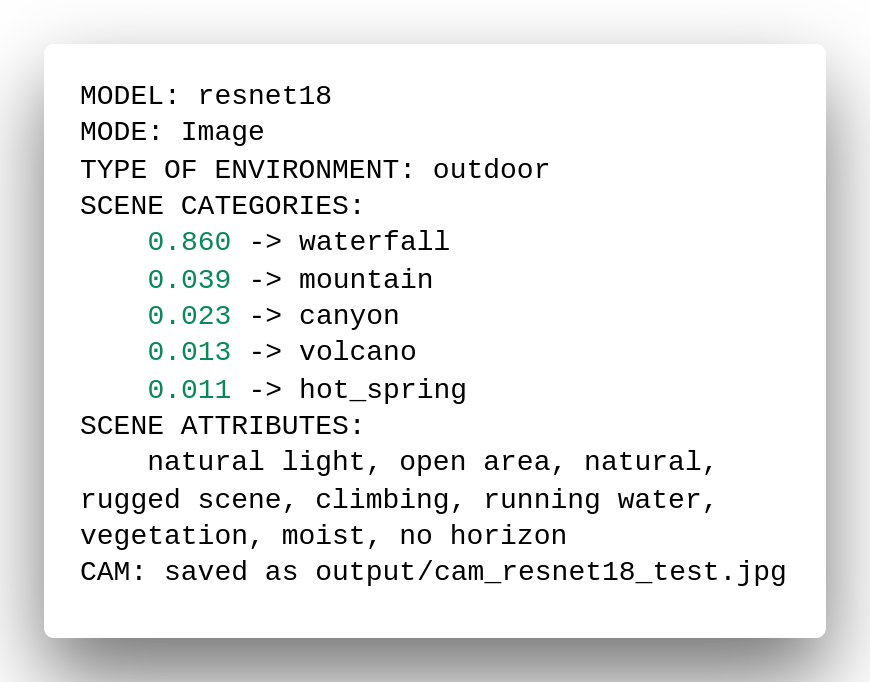
\includegraphics[height=0.3\textheight,keepaspectratio]{week1-places365-resnet18-output.png}
  \caption{Prediction}
\end{subfigure}%
\begin{subfigure}{0.3\textwidth}
  \centering
  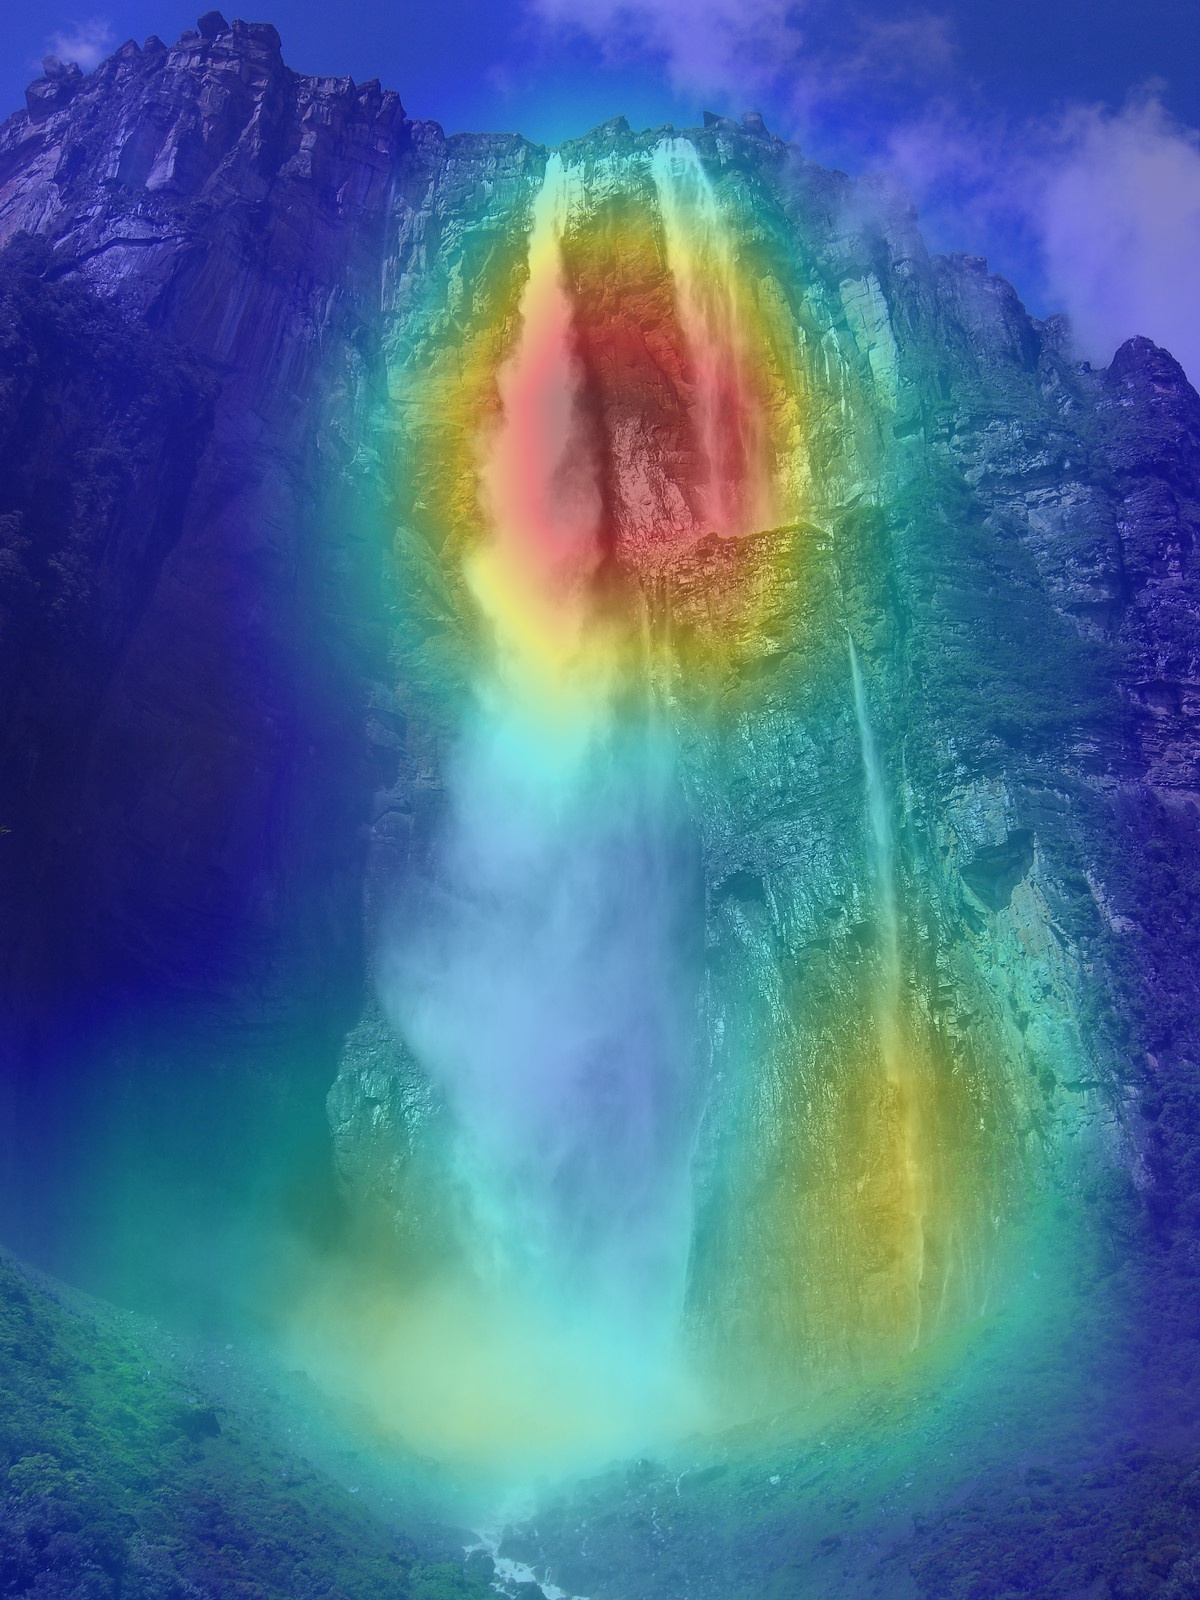
\includegraphics[height=0.3\textheight,keepaspectratio]{week1-cam_resnet18_test.jpg}
  \caption{Class Activation Map}
\end{subfigure}
\caption{Result on ResNet18}
\end{figure}

\begin{figure}[!ht]
\centering
\begin{subfigure}{0.7\textwidth}
  \centering
  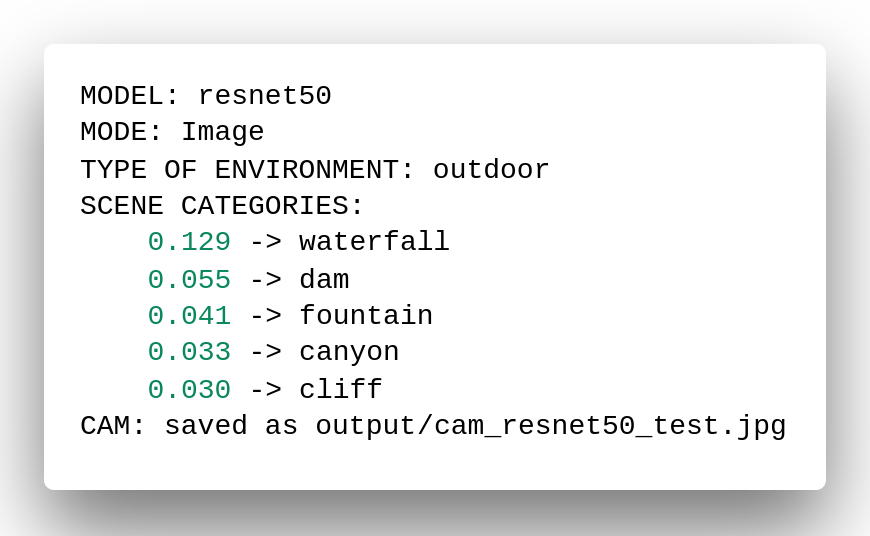
\includegraphics[height=0.24\textheight,keepaspectratio]{week1-places365-resnet50-output.png}
  \caption{Prediction}
\end{subfigure}%
\begin{subfigure}{0.3\textwidth}
  \centering
  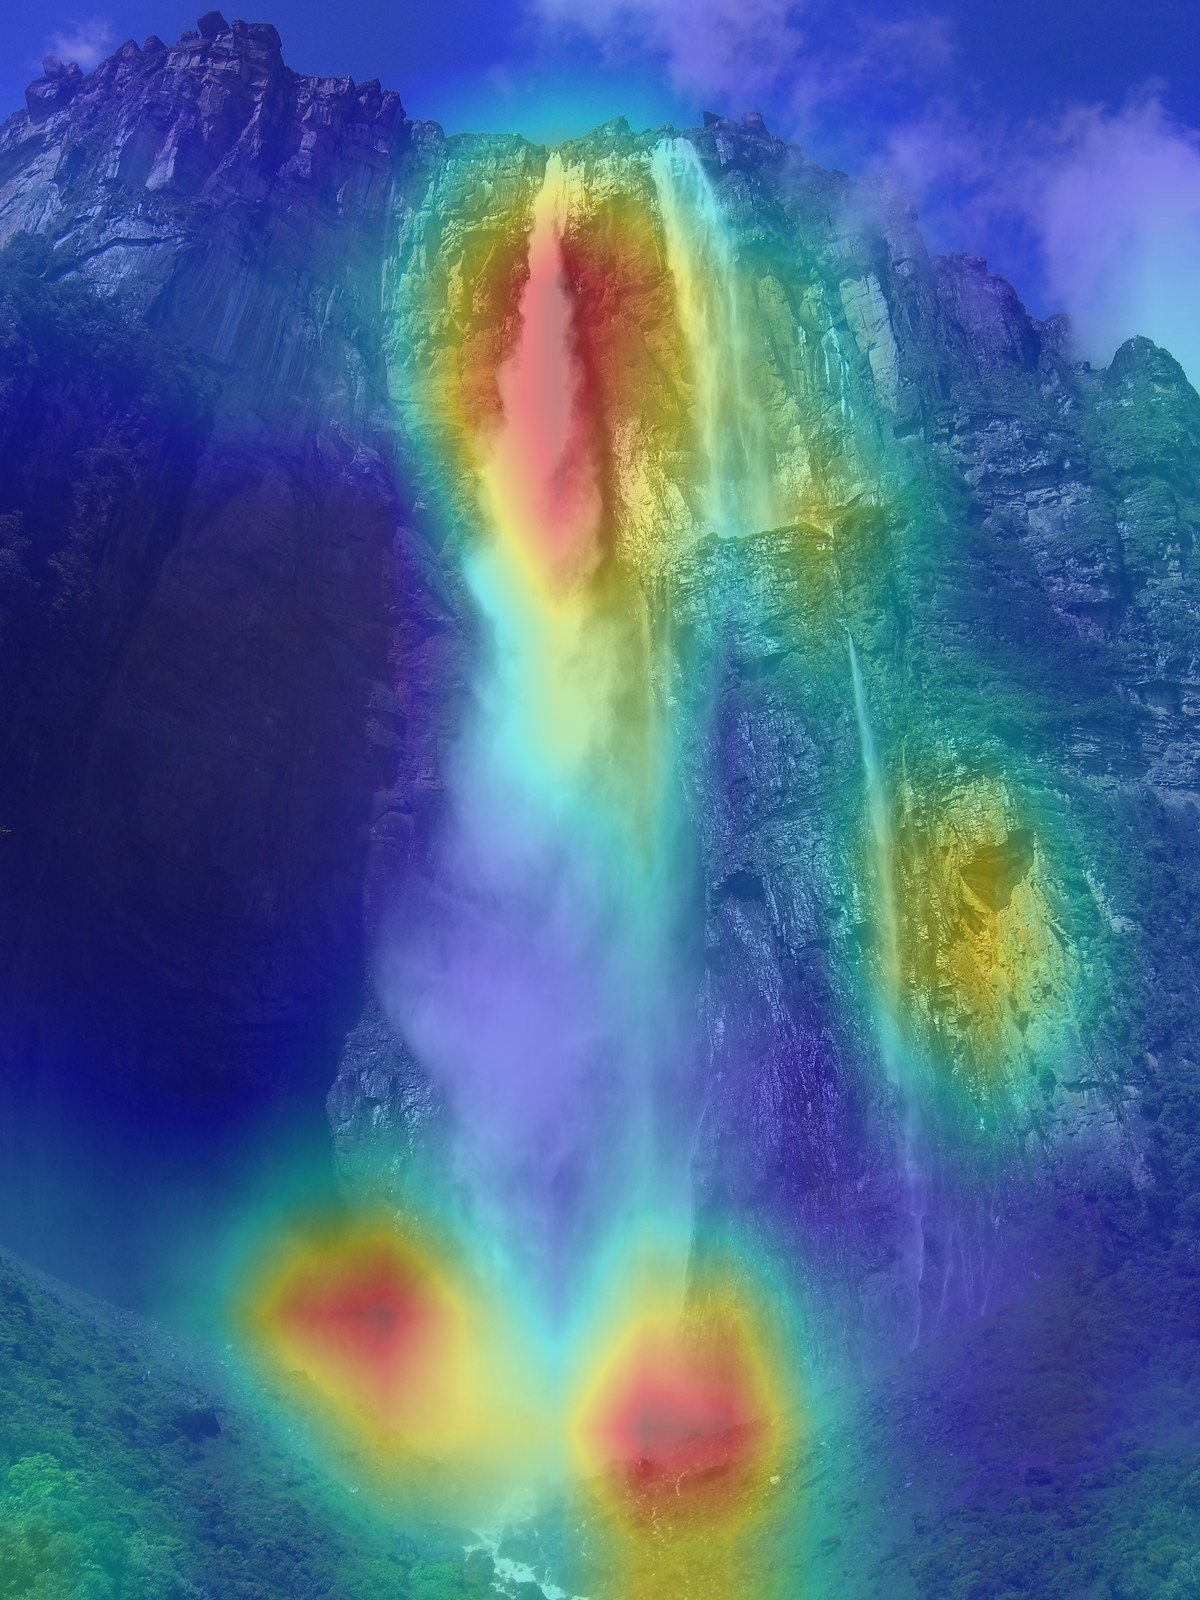
\includegraphics[height=0.3\textheight,keepaspectratio]{week1-cam_resnet50_test.jpg}
  \caption{Class Activation Map}
\end{subfigure}
\caption{Result on ResNet50}
\end{figure}

\newpage
\begin{figure}[!ht]
\centering
\begin{subfigure}{0.7\textwidth}
  \centering
  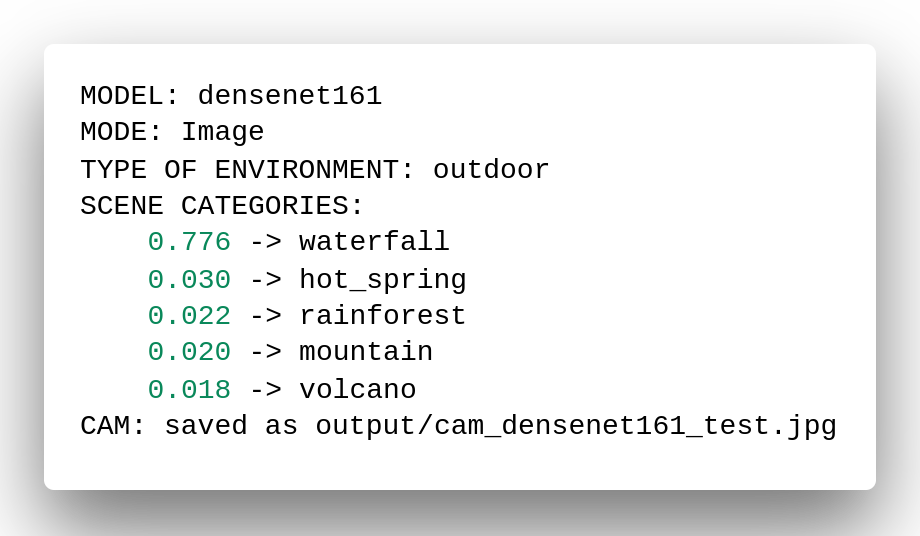
\includegraphics[height=0.23\textheight,keepaspectratio]{week1-places365-densenet161-output.png}
  \caption{Prediction}
\end{subfigure}%
\begin{subfigure}{0.3\textwidth}
  \centering
  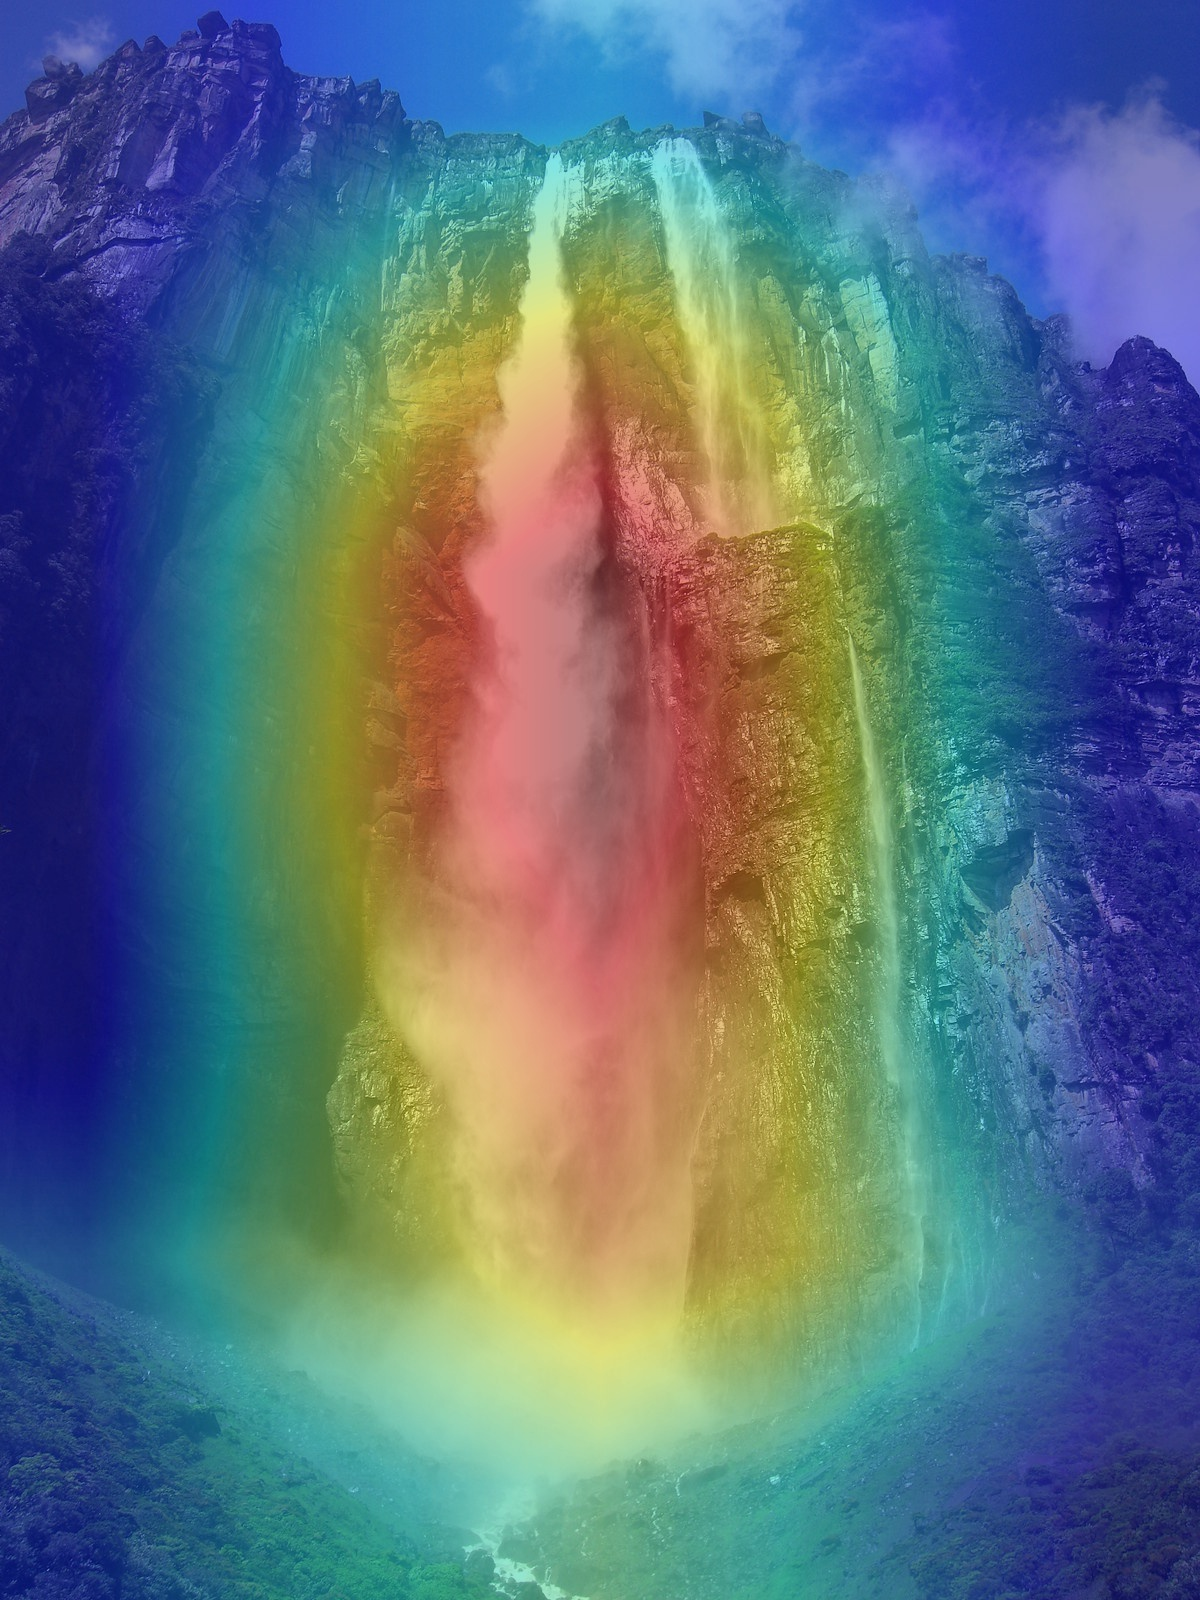
\includegraphics[height=0.3\textheight,keepaspectratio]{week1-cam_densenet161_test.jpg}
  \caption{Class Activation Map}
\end{subfigure}
\caption{Result on DenseNet161}
\end{figure}


\subsection{Source code}
In order to perform tests quickly and efficiently, I rewritten the code from CSAIL to support changing Models, Input type via arguments. My source code could found \href{https://github.com/tlvu2697/places365/blob/tlvu2697/run_placesCNN_args.py}{here on my GitHub}.

\begin{figure}[!ht]
\centering
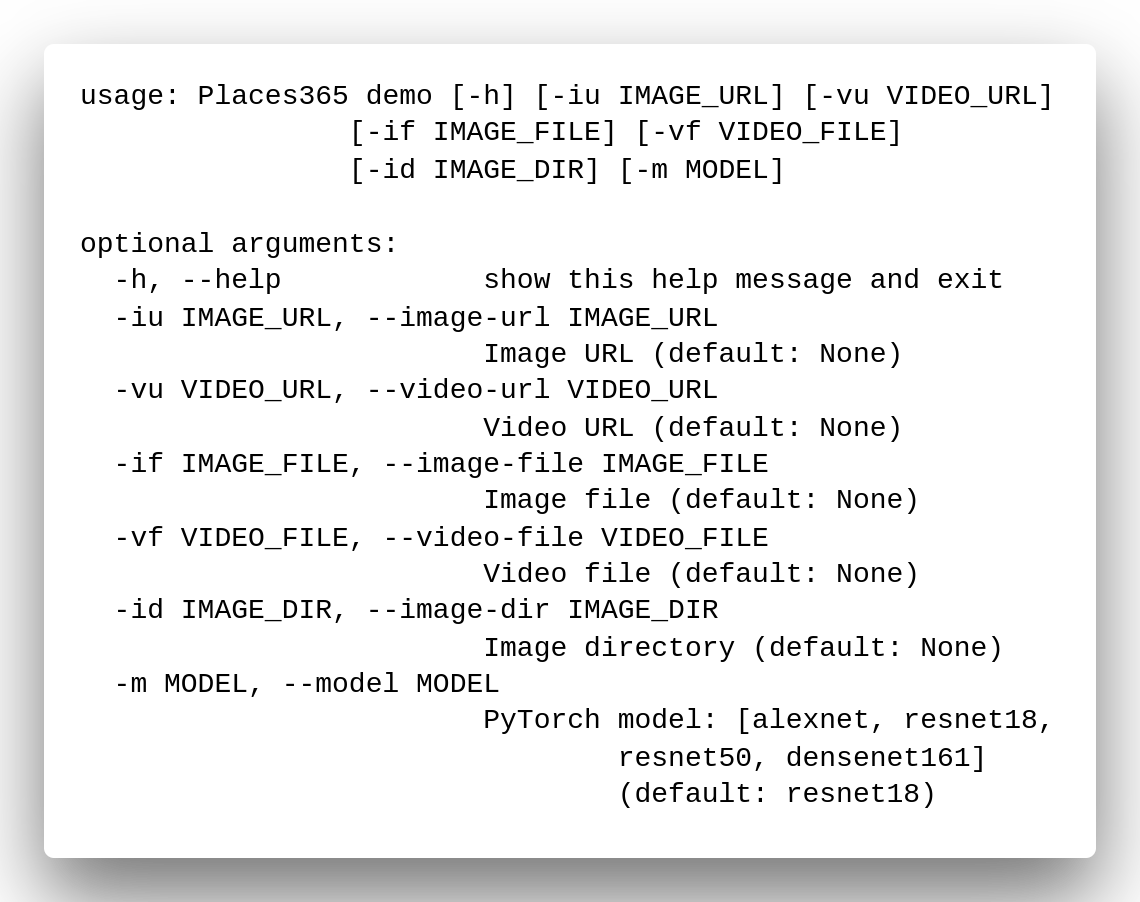
\includegraphics[width=\textwidth,keepaspectratio]{week1-places365-code.png}
\caption{Usage helper}
\end{figure}

\subsection{Class Activation Map}
The authors proposed a simple technique to expose the implicit attention\cite{cam} of Convolutional Neural Networks on the image. The algorithm would highlighted the most informative image regions relevant to the predicted class. This work was published in CVPR'16. The authors also provided example code for testing purpose which could be found \href{https://github.com/metalbubble/CAM}{here on their Github}.

\begin{figure}[!ht]
\centering
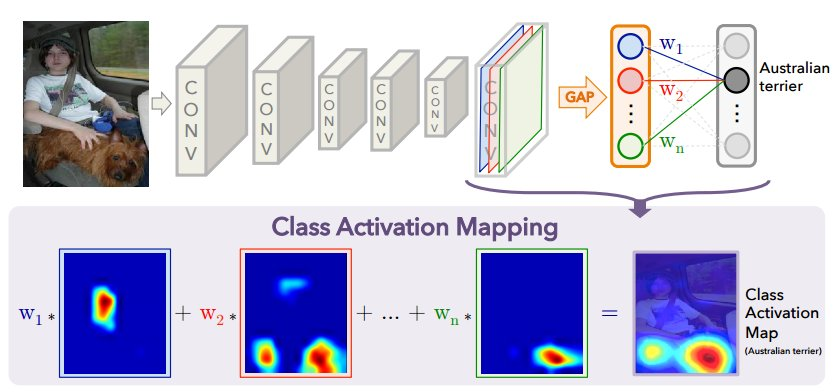
\includegraphics[width=\textwidth,keepaspectratio]{week1-cam-method.jpg}
\caption{The framework of the Class Activation Mapping}
\end{figure}

The technique could be described as: for example we were running on the Resnet, first we had to capture the weight of the penultimate layer of the pre-trained network which could be the Softmax layer; secondly we forwarded our input image through the network; third we captured the output of the last layer right before Convolutional layers, in our case it was the Pooling layer; then we multiplied 2 factors above; finally we represent the result from the previous step onto our input image to get the Class Activation Map. This technique worked similarly for other Convolutional Neral Networks.

As mentioned above, the name of the last layer right before a bunch of Convolutional layers could be different in each Convolutional Neural Network. Its name could be  \emph{features} in the GoogleNet\cite{googlenet} and the DenseNet, \emph{layer4} in the Resnet. Based on our purpose we had to choose the network and the right layers for the Class Activation Mapping algorithm to work properly.

By reading the implementation of these techniques proposed by the author, I had more experience about the architecture of a Torchvision model and how to explore a neural network. Using the \emph{\_modules} variable to explore the whole architecture (layer by layer) of that neural network and the \emph{register-forward-hook} function to hook the parameters of a concrete layer during the forward pass; these two techniques helped me extracting the features of an input images. As the result, I was able to convert images to vectors by using any pre-trained Convolutional Neural Network (e.g. ResNet, Inception v3, DenseNet, ...).